\documentclass[20pt]{beamer}
\usepackage[utf8]{inputenc}
\usepackage[utf8]{vietnam}
\usepackage{amsmath}
\usepackage{amsfonts}
\usepackage{amssymb}
\usepackage{graphicx}
\usepackage{xcolor}
\usepackage{utopia} %font utopia imported

\usepackage{ragged2e}
\usepackage{etoolbox}

\mode<beamer>{\usetheme{CambridgeUS}}

\usecolortheme{default}

\usepackage{hyperref}
\hypersetup{pdfpagemode=FullScreen} %mode FullScreen with beamer

\apptocmd{\frame}{}{\justifying}{} % Allow optional arguments after frame.

\usepackage{comment}

\makeatletter
\let\insertuniversity\relax
\newcommand\universitytitle{TRƯỜNG ĐH}

\let\insertclass\relax
\newcommand\classtitle{Lớp}

\let\insertcourse\relax
\newcommand\coursetitle{Môn học}

\mode<all>
{
  \newcommand\university[1]{\def\insertuniversity{#1}}
  
  \newcommand\class[1]{\def\insertclass{#1}}
  
  \newcommand\course[1]{\def\insertcourse{#1}}
  \titlegraphic{}
}

\defbeamertemplate*{title page}{supdefault}[1][]
{
  \begingroup
    \centering
    \ifx\insertuniversity\relax\relax\else
    \begin{beamercolorbox}[sep=2pt,center,#1]{author}
      \footnotesize\universitytitle~\insertuniversity
    \end{beamercolorbox}\fi
    
    \begin{beamercolorbox}[sep=8pt,center,#1]{title}
      \usebeamerfont{title}\large\inserttitle\par%
      \ifx\insertsubtitle\@empty\relax%
      \else%
        \vskip0.25em%
        {\usebeamerfont{subtitle}\usebeamercolor[fg]{subtitle}\insertsubtitle\par}%
      \fi%     
    \end{beamercolorbox}%
    \vskip.5em\par

    \vspace{-.3cm}
    \ifx\insertcourse\relax\relax\else
    \begin{beamercolorbox}[sep=6pt,center,#1]{author}
      \usebeamerfont{author}\small\coursetitle:~\insertcourse
    \end{beamercolorbox}\fi

    \vspace{-.3cm}
    \ifx\insertclass\relax\relax\else
    \begin{beamercolorbox}[sep=6pt,center,#1]{author}
      \usebeamerfont{author}\small\classtitle:~\insertclass
    \end{beamercolorbox}\fi

    \vspace{-.3cm}
    \begin{beamercolorbox}[sep=6pt,center,#1]{author}
      \usebeamerfont{author}\small\insertauthor
    \end{beamercolorbox}
    %\begin{beamercolorbox}[sep=8pt,center,#1]{institute}
      %\usebeamerfont{institute}\insertinstitute
    %\end{beamercolorbox}
    \vspace{-.3cm}
    \begin{beamercolorbox}[sep=8pt,center,#1]{date}
      \usebeamerfont{date}\small\insertdate
    \end{beamercolorbox}\vskip0.5em
    {\usebeamercolor[fg]{titlegraphic}\inserttitlegraphic\par}
  \endgroup
  \vfill
}
\setbeamertemplate{title page}[supdefault][colsep=-4bp,rounded=true,shadow=\beamer@themerounded@shadow]\makeatother

%Title page
\title[Động cơ không đồng bộ]{\emph{Chủ đề báo cáo}\\Khởi động mềm và Phương pháp thay đổi tốc độ động cơ KĐB}
\author[Cơ sở Truyền động điện]{GVHD: Hồ Minh Nhị \and Nhóm SVTH: Nhóm 1}
\course{Cơ sở Truyền động điện}
\class{Công nghệ, kỹ thuật điện, điện tử}
\university{KỸ THUẬT -- CÔNG NGHỆ CẦN THƠ}
\date[Nhóm 1]{\today}
%\date[Nhóm 1]{Ngày 24 tháng 08 năm 2016}

%\logo{
\includegraphics[height=1.3cm]{logo_ctut.pdf}}

\AtBeginSection[]
{
  \begin{frame}
    \frametitle{Nội dung báo cáo}
    \justifying
    \tableofcontents[currentsection]
  \end{frame}
}
\definecolor{doden}{RGB}{204, 0, 0}
\begin{document}
%http://tex.stackexchange.com/questions/82794/removing-page-number-from-title-frame-without-changing-the-theme
\bgroup
\makeatletter
\setbeamertemplate{footline}
{
  \leavevmode%
  \hbox{%
  \begin{beamercolorbox}[wd=.333333\paperwidth,ht=2.25ex,dp=1ex,center]{author in head/foot}%
    \usebeamerfont{author in head/foot}\insertshortauthor\expandafter\beamer@ifempty\expandafter{\beamer@shortinstitute}{}{~~(\insertshortinstitute)}
  \end{beamercolorbox}%
  \begin{beamercolorbox}[wd=.333333\paperwidth,ht=2.25ex,dp=1ex,center]{title in head/foot}%
    \usebeamerfont{title in head/foot}\insertshorttitle
  \end{beamercolorbox}%
  \begin{beamercolorbox}[wd=.333333\paperwidth,ht=2.25ex,dp=1ex,right]{date in head/foot}%
    \usebeamerfont{date in head/foot}\insertshortdate{}\hspace*{2em}
%    \insertframenumber{} / \inserttotalframenumber\hspace*{2ex} 
    \hspace*{6ex}
  \end{beamercolorbox}}%
  \vskip0pt%
}

\begin{frame}
\titlepage
\end{frame}
\egroup

\setcounter{framenumber}{0}

%--------------------------------------------------------------------------------
%--------------------------------------------------------------------------------
% Danh sach thanh vien
\begin{frame}{Danh sách thành viên}
	\vspace{-1cm}
	\begin{small}
	\begin{columns}
		\column{0.6\textwidth}
		\begin{enumerate}
			\item Nguyễn Văn Bảy
			\item Nguyễn Văn Đình
			\item Nguyễn Hoàng Hận
			\item Thi Minh Nhựt
			\item Phạm Thanh Quý
			\item Hồ Minh Thành
			\end{enumerate}

		\column{0.6\textwidth}
		\begin{enumerate}	% Danh sach tiep theo
			\setcounter{enumi}{6}
			\item Nguyễn Văn Tiến
			\item Liên Thái Trường
			\item Trần Thanh Tú
			\item Bùi Trọng Tuấn
			\item Lư Anh Tuấn
			\item Nguyễn Bá Vọng
		\end{enumerate}
	\end{columns}
	\end{small}
\end{frame}

%--------------------------------------------------------------------------------
%--------------------------------------------------------------------------------
% Noi dung bao cao
\begin{frame}	%Trang muc luc
	\frametitle{Nội dung báo cáo}
	\tableofcontents
\end{frame}

\section{Khởi động mềm động cơ KĐB ba pha}
%--------------------------------------------------------------------------------
%--------------------------------------------------------------------------------
% Khởi động mềm động cơ 3 pha
\subsection*{Sơ đồ nguyên lý}
\begin{frame}{Bộ khởi động mềm}
	\vspace{-1.5cm}
	\begin{center}
		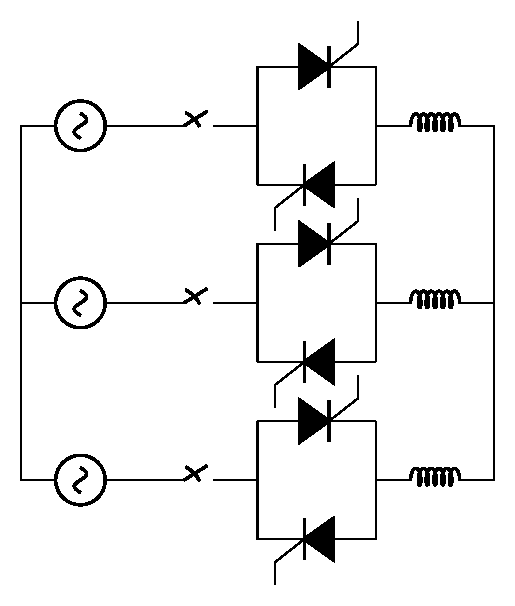
\includegraphics[scale=.8,angle=-90]{../sodomach/khoidongmem.pdf} 
	\end{center}
\end{frame}

\subsection*{Đặc điểm}
\begin{frame}{Bộ khởi động mềm}
	\begin{block}{Đặc điểm}
		\begin{list}{--}{}
			\justifying
			\item Thay đổi điện áp, giữ nguyên tần số. 
			\item Dừng tự do theo quán tính, dừng mềm, tiết kiệm năng lượng khi non tải.
		\end{list}
	\end{block}
\end{frame}

\begin{frame}{Bộ khởi động mềm}
	\begin{block}{Ưu điểm}
		\begin{list}{--}{}
			\justifying
			\item Điều chỉnh trơn, phạm vi điều chỉnh rộng, hoạt động ổn định,\ldots
			\item Tránh sụt áp khi khởi động, tích hợp nhiều mạch bảo vệ động cơ,\ldots
			\item Hạn chế được dòng khởi động và điều chỉnh được moment mở máy.
		\end{list}
	\end{block}
\end{frame}

\begin{frame}{Bộ khởi động mềm}
	\justifying	
	\begin{block}<1->{Nhược điểm}
		Khó thi công, bão dưỡng, điện áp, dòng điện điều chỉnh không $\sin$, bị méo, biên độ sóng hài cao,\ldots
	\end{block}
	\begin{block}<2->{Phạm vi áp dụng}
		ĐC công suất trung bình và lớn.
	\end{block}
\end{frame}


%--------------------------------------------------------------------------------
%--------------------------------------------------------------------------------
% Các phương pháp thay đổi tốc độ động cơ
\section[Thay đổi tốc độ động cơ KĐB ba pha]{Phương pháp thay đổi tốc độ động cơ KĐB ba pha}

%--------------------------------------------------------------------------------
% Tốc độ động cơ KĐB
\subsection*{Tốc độ động cơ KĐB}
\begin{frame}{Tốc độ của động cơ KĐB}
	\begin{block}<1->{Tốc độ quay}
		$$ n = \left({1-s}\right)n_1 = \left({1-s}\right) \dfrac{60f}{p}$$
	\end{block}

	\begin{block}<2->{Nhận xét}
		\justifying
		Tốc độ đồng cơ KĐB phụ thuộc vào: $\textcolor{doden}{s}$, $\textcolor{doden}{f}$, $\textcolor{doden}{p}$.
	\end{block}
\end{frame}

%--------------------------------------------------------------------------------
% Phương pháp thay đổi tốc độ
\subsection*{Phương pháp thay đổi tốc độ}
\begin{frame}[t]{Phương pháp thay đổi tốc độ ĐC KĐB}
	\begin{itemize}
		\item Thay đổi tần số nguồn cấp stator.
		\item Thay đổi cặp cực dây quấn stator.
		\item Điều chỉnh điện áp stato.
		\item Thay đổi điện trở mạch roto.
	\end{itemize}
\end{frame}

%--------------------------------------------------------------------------------
% Thay đổi số cặp cực
\subsection*{Thay đổi số cặp cực}
\begin{frame}{Thay đổi số cặp cực}
	\begin{figure}
		\begin{center}
			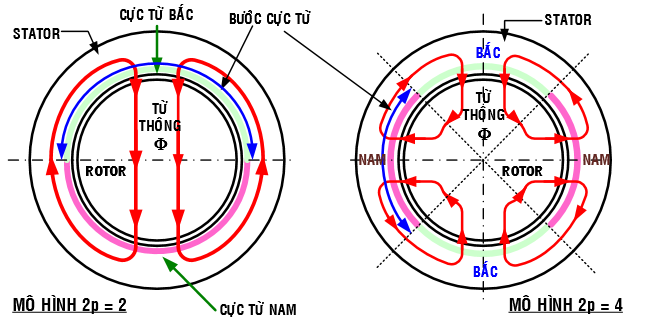
\includegraphics[scale=.55]{images-chude2/2-and-4-pole-AC3P.png} 
		\end{center}
		\caption{Mô hình số cặp cực của ĐC KĐB}
	\end{figure}
\end{frame}

\begin{frame}{Thay đổi số cặp cực}
	\begin{block}<1->{Biện pháp}
		Thay đổi \textcolor{doden}{cấu tạo dây quấn}.
   \end{block}
   
   \begin{block}<2->{Phạm vi áp dụng}
		Chỉ áp dụng cho động cơ \textcolor{doden}{rotor lồng sóc}.
   \end{block}
   
   \begin{block}<3->{Nhận xét}
		Khi \textcolor{doden}{tăng số cặp cực} $\longrightarrow$ \textcolor{doden}{tốc độ giảm}.
   \end{block}
\end{frame}

\begin{frame}{Thay đổi số cặp cực}
	\begin{block}<1->{Ưu điểm}
		\justifying
		Đơn giản, rẻ tiền, giữ nguyên độ cứng cơ, thay đổi tốc độ triệt để,\ldots
   \end{block}
   
   \begin{block}<2->{Nhược điểm}
   		\justifying
		Độ tin cậy kém, dãi điều chỉnh tốc độ hẹp, kích thước động cơ lớn,\ldots
   \end{block}
\end{frame}

%--------------------------------------------------------------------------------
% Thay đổi điện áp stator
\subsection*{Thay đổi điện áp stator}
\begin{frame}{Thay đổi điện áp vào stator}
	\vspace{-3.3cm}
	\begin{center}
		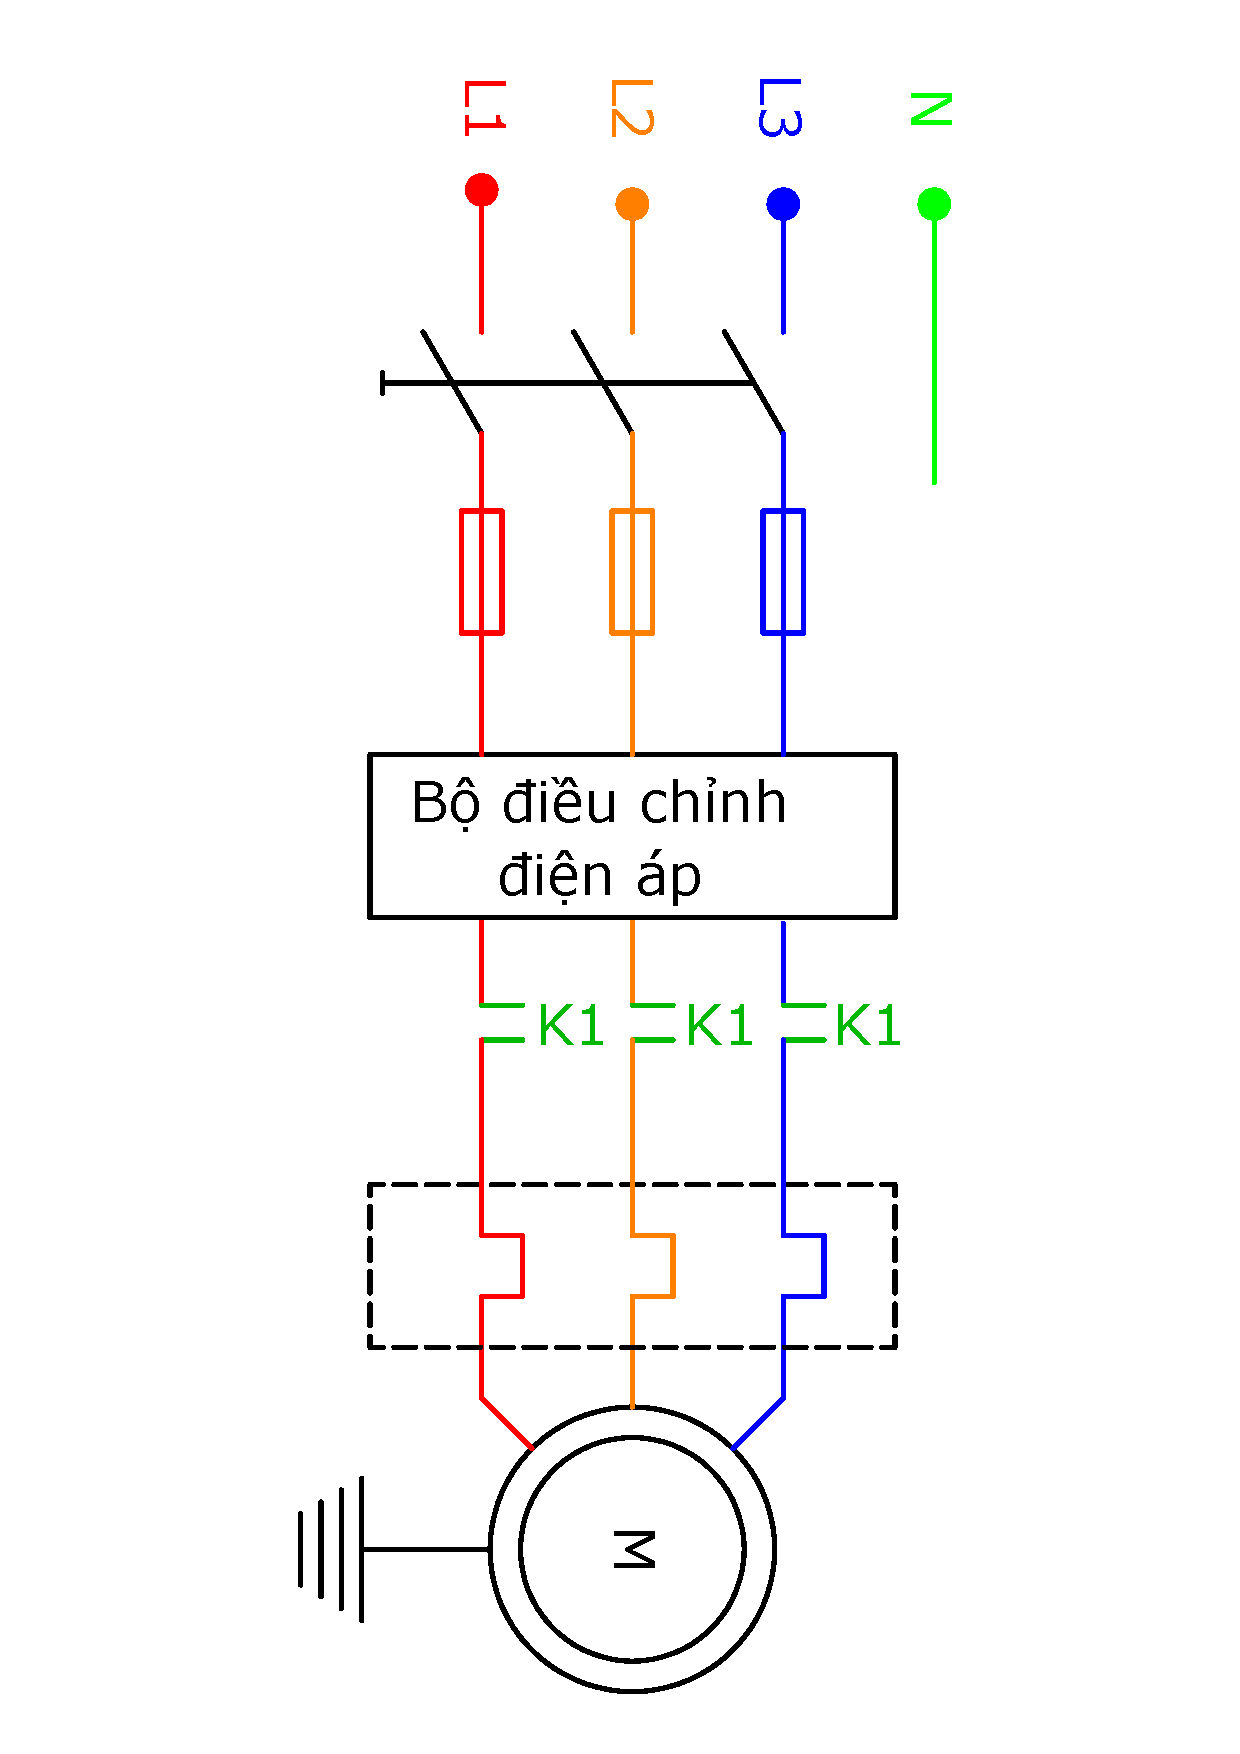
\includegraphics[scale=0.4, angle = 90]{../sodomach/dieu-chinh-dien-ap-stator.pdf}
	\end{center}
	\vspace{-3cm}
	\begin{block}{Phạm vi áp dụng}
		ĐC đang mang tải.
	\end{block}
\end{frame}

\begin{frame}{Thay đổi điện áp vào stator}
	\begin{block}<1->{Mục đích}
		\justifying
		Thay đổi \textcolor{doden}{hệ số trượt $s$} $\longrightarrow$ thay đổi \textcolor{doden}{tốc độ $n$ của động cơ}.
   \end{block}
   
   \begin{block}<2->{Nhận xét}
   		\justifying
		Khi \textcolor{doden}{tăng điện áp} $\longrightarrow$ \textcolor{doden}{hệ số trượt giảm} $\longrightarrow$ \textcolor{doden}{tốc độ đông cơ tăng}.
   \end{block}
\end{frame}

\begin{frame}{Thay đổi điện áp vào stator}
	\begin{block}<1->{Ưu điểm}
		\justifying
		Thực hiện dễ dàng, sử dụng rộng rãi,\ldots
   \end{block}
   
   \begin{block}<2->{Nhược điểm}
   		\justifying
   		Giảm khả năng quá tải, tổn hao trong rotor,\ldots
   \end{block}
\end{frame}

%--------------------------------------------------------------------------------
% Thay đổi điện trở mạch rotor
\subsection*{Thay đổi điện trở mạch rotor}
\begin{frame}{Thay đổi điện trở mạch rotor}
	\vspace{-2.5cm}
	\begin{center}
		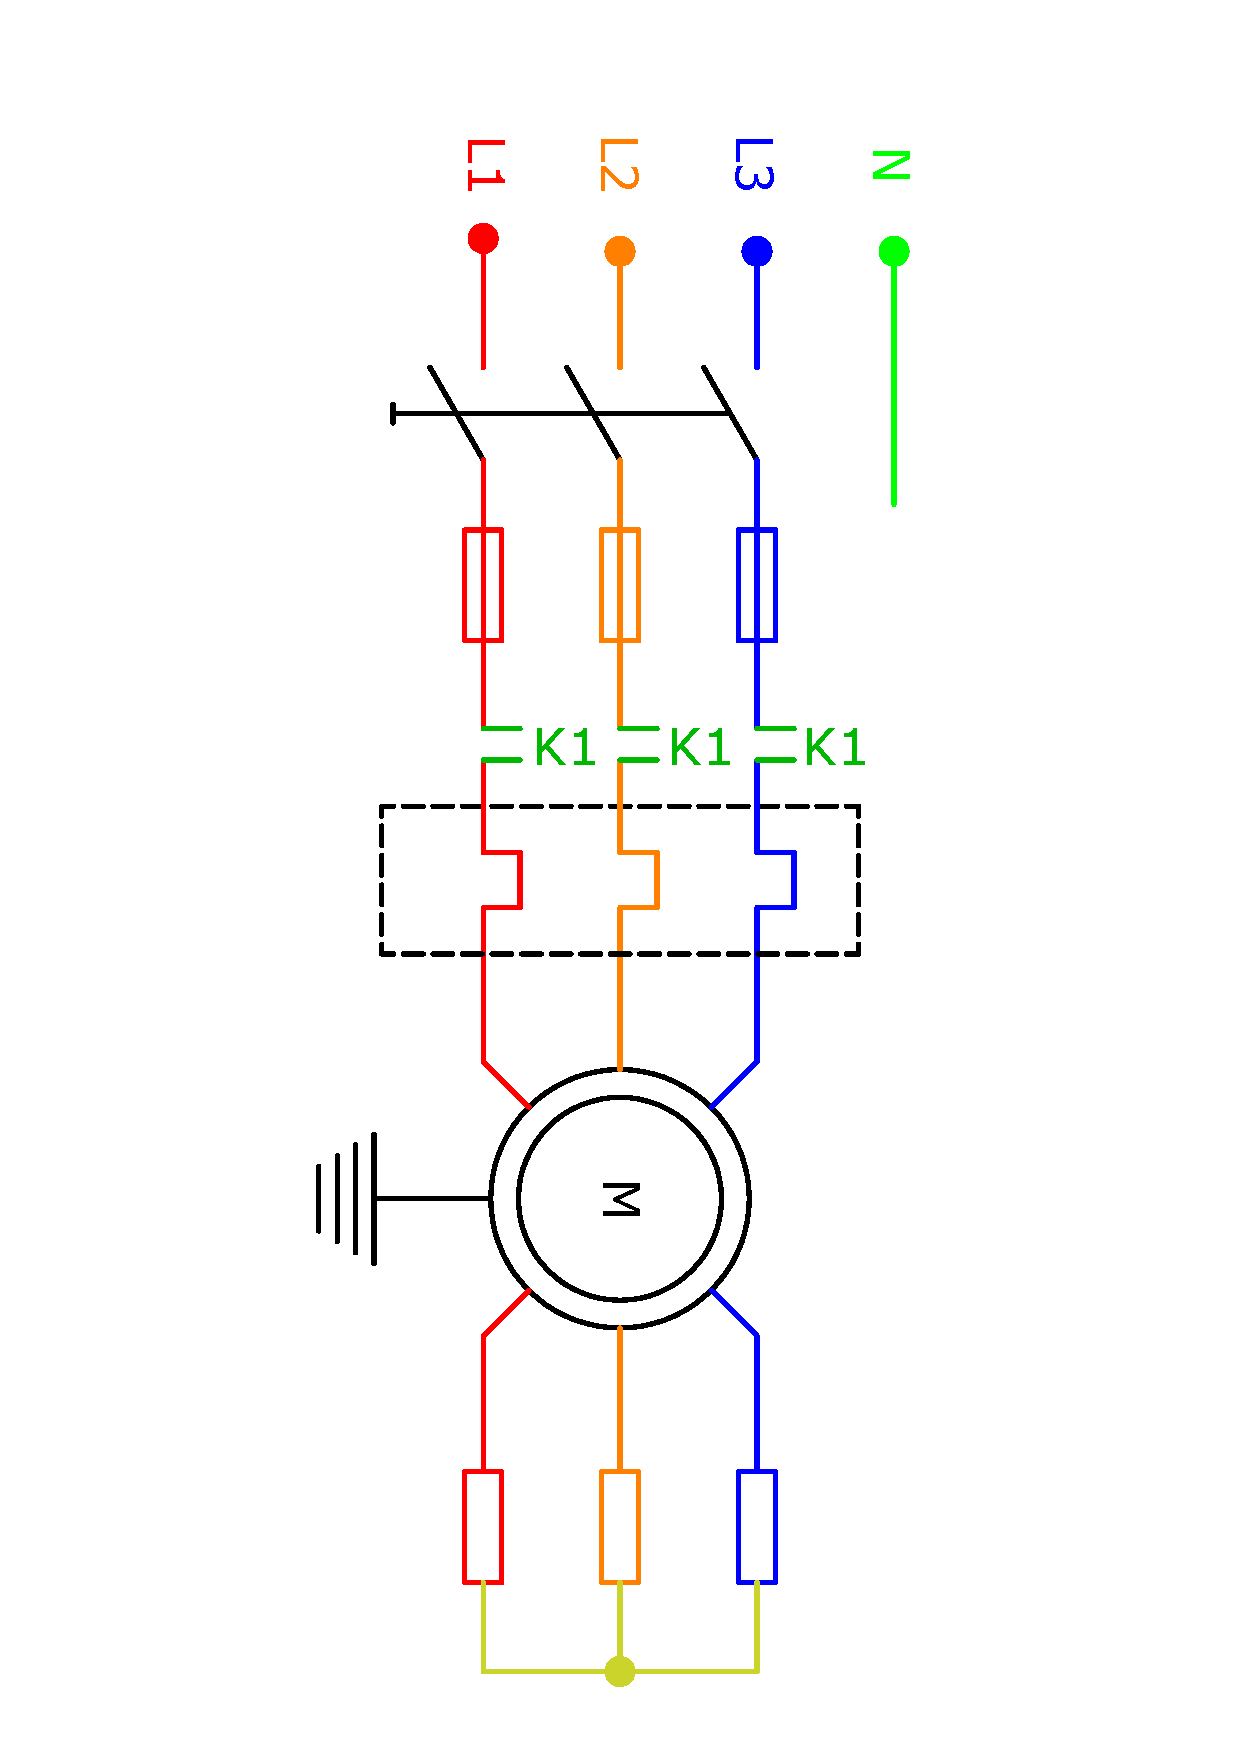
\includegraphics[scale=0.4, angle = 90]{../sodomach/dieu-chinh-dien-tro-rotor.pdf}
	\end{center}
\end{frame}

\begin{frame}{Thay đổi điện trở mạch rotor}
	\begin{block}<1->{Phạm vi áp dụng}
		\justifying
		ĐC rotor dây quấn, công suất cỡ trung bình, các ứng dụng truyền động ngắn hạn.
	\end{block}

	\begin{block}<2->{Nhận xét}
		\textcolor{doden}{Tăng điện trở} $\longrightarrow$ \textcolor{doden}{tốc độ động cơ giảm}.
	\end{block}
\end{frame}

\begin{frame}{Thay đổi điện trở mạch rotor}
	\begin{block}<1->{Ưu điểm}
		\justifying
		Đơn giản, điều chỉnh trơn, khoảng điều chỉnh rộng.
	\end{block}
	
	\begin{block}<2->{Nhược điểm}
		\justifying
		Tổn hao công suất trên điện trở, không kinh tế,\ldots
	\end{block}
\end{frame}

%--------------------------------------------------------------------------------
%--------------------------------------------------------------------------------
% Tai lieu tham khao
\section*{Tài liệu tham khảo}
\begin{frame}{Tài liệu tham khảo}
\justifying
[1]. Nguyễn Văn Nhờ, \textit{Cơ sở Truyền động điện}, NXB ĐH Quốc gia HCM.

[2]. Đặng Văn Đào, Lê Văn Doanh -- \textit{Kỹ thuật điện}, NXB: ĐH Khoa học và Kỹ thuật

[3]. \href{http://maynenkhitrucvit.com.vn/index.php/ky-thuat/50-dong-co-may-nen-khi/81-phuong-phap-dieu-chinh-toc-do-dong-co-khong-dong-bo.html}{Phương  pháp điều chỉnh tốc độ ĐC KĐB}
\end{frame}
%https://2bientan.wordpress.com/2015/03/31/khoi-dong-mem-la-gi-tai-lieu-va-nguyen-ly-khoi-dong-mem/
%--------------------------------------------------------------------------------
%--------------------------------------------------------------------------------
% Tai lieu tham khao
\section*{Lời cảm ơn}
\begin{frame}
\justifying
\large \alert{Cảm ơn Thầy và các bạn đã quan tâm theo dõi phần trình bày của nhóm!}
\end{frame}
\end{document}